\documentclass[11pt]{article}

\usepackage[margin=1in]{geometry}
\usepackage{amsmath,amssymb}
\usepackage{booktabs}
\usepackage{graphicx}
\usepackage{hyperref}
\usepackage[numbers,sort&compress]{natbib}
\usepackage{url}

\title{Descriptor-Teacher Guided Multi-to-Uni Transfer for Low-Resource Regression ADMET Prediction}
\author{Yuzibo\\\small Affiliation to be finalized}
\date{}

\begin{document}
\maketitle

\begin{abstract}
Low-resource ADMET prediction is a recurring challenge in early-stage drug
discovery, where labeled assays are limited but inexpensive molecular knowledge
such as physicochemical descriptors is readily available. We study whether
descriptor knowledge can be transferred into an ECFP-only neural predictor, so
that descriptors guide training without being required at inference time. We
develop Descriptor-Teacher AdapterFusion, a lightweight ECFP4-based student
model that combines an adapter-based pseudo-descriptor representation with
descriptor reconstruction and teacher prediction distillation from an
ECFP4+descriptor random forest. Across five regression ADMET datasets, three
low-resource training ratios, and three random seeds, fixed teacher
distillation with $\lambda_{\mathrm{distill}}=1.0$ improves AdapterFusion in
11/15 dataset-ratio settings, with an average RMSE change of -0.0656 relative
to the undistilled AdapterFusion baseline. Descriptor-access random forest
models remain stronger in most settings, so the contribution is controlled
descriptor knowledge transfer rather than an overall ADMET state-of-the-art
claim. A lambda sweep and adaptive-weighting ablation further show that simple
validation-based adaptive distillation is not sufficient.
\end{abstract}

\section{Introduction}

Accurate ADMET prediction is important for early drug discovery because
absorption, distribution, metabolism, excretion, and toxicity properties affect
which candidate molecules can progress beyond screening
\citep{Vamathevan2019,Butler2018,Xiong2021ADMETlab}. Many ADMET tasks are
low-resource: labels are expensive to obtain, measurements vary across assays,
and each property may have a limited number of reliable annotated compounds.
This makes it useful to study lightweight models and auxiliary molecular
knowledge that can improve generalization under limited supervision.

Molecular descriptors provide one such source of auxiliary knowledge. RDKit
physicochemical descriptors are inexpensive to compute and often correlate with
ADMET behavior \citep{RDKit2026}. A direct way to exploit them is to
concatenate descriptors with molecular fingerprints or use descriptor-based
traditional models. However, this creates a descriptor-access inference
setting. In contrast, a multi-to-uni transfer setting asks whether descriptor
knowledge can be used during training while the deployed model uses only a
single modality, here ECFP4 fingerprints \citep{Rogers2010}.

This paper studies descriptor-guided multi-to-uni transfer for low-resource
ADMET prediction. We begin from an ECFP4 MLP baseline, compare simple auxiliary
descriptor prediction with a structured AdapterFusion student, and then add
teacher prediction distillation from an ECFP4+descriptor random forest. Our
central question is deliberately narrow: can descriptor-access knowledge
improve an ECFP-only student in low-resource regression ADMET? The answer is
positive but bounded. Teacher distillation improves AdapterFusion in most
regression settings, but descriptor-access random forest baselines remain
strong.

The contributions are:
\begin{itemize}
  \item We formulate a lightweight descriptor-guided multi-to-uni transfer
  setup for low-resource ADMET prediction.
  \item We compare ECFP-only descriptor prediction, AdapterFusion,
  descriptor-access controls, random forest baselines, and teacher-distilled
  AdapterFusion under shared low-resource splits.
  \item We show that fixed descriptor-teacher distillation improves regression
  AdapterFusion in 11/15 dataset-ratio settings.
  \item We report lambda sensitivity, validation-selected lambda analysis, and
  a negative adaptive-weighting ablation.
\end{itemize}

\section{Related Work}

Molecular representation learning has increasingly used auxiliary objectives
to inject chemical knowledge into learned representations. Molecular language
models such as MolBERT motivate the use of domain-relevant pretraining or
auxiliary tasks rather than relying only on generic representation learning
objectives \citep{Fabian2020MolBERT}. Graph pretraining methods such as GNN
pretraining, GROVER, and GraphMVP similarly use self-supervised or cross-view
objectives to improve downstream molecular prediction
\citep{Hu2020PretrainGNN,Rong2020GROVER,Liu2022GraphMVP}. Our work is smaller
in scale and does not use a large pretrained encoder, but it shares the
principle that chemically meaningful auxiliary targets can shape molecular
representations.

Auxiliary learning and task-specific adaptation are also relevant. A simple
auxiliary objective may not transfer all useful knowledge to the downstream
task; the architecture through which auxiliary information is routed can matter
\citep{Ruder2017,Dey2024AuxAdapt}. The closest conceptual motivation is
multi-to-uni molecular representation learning, including M2UMol-style
knowledge transfer \citep{Xiong2026M2UMol}. Our setting is deliberately
controlled: descriptors are the auxiliary modality, ECFP4 is the inference
modality, and ADMET prediction is the downstream task.

ADMET benchmark modeling provides the application context. We use TDC-style
ADMET datasets and evaluate low-resource splits across regression and
classification properties \citep{Huang2021TDC}. MoleculeNet provides an earlier
benchmarking reference for molecular property prediction metrics, splits, and
baselines \citep{Wu2018MoleculeNet}. Fingerprint and descriptor models remain
important controls in cheminformatics, while graph neural networks and directed
message-passing models provide stronger learned-representation baselines in
larger studies
\citep{Kearnes2016GraphConv,Yang2019DMPNN,Xiong2020AttentiveFP,Heid2024Chemprop}.
Tree ensembles are included because random forests and gradient boosting
methods remain competitive for tabular molecular features
\citep{Breiman2001,Chen2016XGBoost,Ke2017LightGBM,Tian2022ADMETBoost}.

\section{Method}

\subsection{Problem setting}

Each molecule has an ECFP4 fingerprint $x_{\mathrm{ecfp}}$, an optional
descriptor vector $x_{\mathrm{desc}}$, and a target $y$. The primary inference
constraint is that the student model should use only $x_{\mathrm{ecfp}}$ at
test time. Descriptor information may be used during training as auxiliary
supervision or through teacher predictions. The main paper focuses on
regression tasks, where the task loss is mean squared error.

\subsection{ECFP encoder and descriptor prediction}

The base ECFP model maps a 2048-dimensional ECFP4 fingerprint to a
128-dimensional latent representation using a two-layer MLP:
\begin{equation}
z_{\mathrm{fp}} = f_{\mathrm{fp}}(x_{\mathrm{ecfp}}).
\label{eq:ecfp_encoder}
\end{equation}
The simple descriptor-prediction baseline adds an auxiliary head that predicts
standardized RDKit descriptors from $z_{\mathrm{fp}}$. Its training objective
is:
\begin{equation}
\mathcal{L} =
\mathcal{L}_{\mathrm{task}} +
\lambda_{\mathrm{transfer}}\mathcal{L}_{\mathrm{desc}},
\label{eq:descpred_loss}
\end{equation}
where $\lambda_{\mathrm{transfer}}=0.1$. The descriptor vector contains nine
RDKit descriptors: MolWt, LogP, TPSA, HBA, HBD, rotatable bonds, aromatic ring
count, heavy atom count, and ring count.

\subsection{AdapterFusion student}

The AdapterFusion student uses the same ECFP encoder but introduces a
pseudo-descriptor adapter:
\begin{equation}
z_{\mathrm{desc}} = f_{\mathrm{adapter}}(z_{\mathrm{fp}}).
\label{eq:adapter}
\end{equation}
A learned fusion gate combines the original ECFP representation and the
pseudo-descriptor representation:
\begin{align}
g &= \sigma(f_{\mathrm{gate}}([z_{\mathrm{fp}}, z_{\mathrm{desc}}])),\\
z_{\mathrm{fused}} &= g \odot z_{\mathrm{fp}} + (1-g)\odot z_{\mathrm{desc}}.
\label{eq:fusion}
\end{align}
The target prediction head receives $z_{\mathrm{fused}}$, while the descriptor
prediction head predicts descriptors from $z_{\mathrm{desc}}$. This structure
keeps inference ECFP-only, because no true descriptors are consumed by the
student at test time.

\subsection{Descriptor-teacher distillation}

We include descriptor-access controls to estimate the value of direct
descriptor information. The strongest descriptor-access teacher used here is an
ECFP4+descriptor random forest. The distilled student keeps the AdapterFusion
architecture and adds a teacher prediction loss:
\begin{equation}
\mathcal{L}_{\mathrm{teacher}} =
\mathrm{MSE}(\hat{y}_{\mathrm{student}}, \hat{y}_{\mathrm{teacher}}).
\label{eq:teacher_loss}
\end{equation}
The final objective is:
\begin{equation}
\mathcal{L} =
\mathcal{L}_{\mathrm{task}} +
\lambda_{\mathrm{transfer}}\mathcal{L}_{\mathrm{desc}} +
\lambda_{\mathrm{distill}}\mathcal{L}_{\mathrm{teacher}}.
\label{eq:distill_loss}
\end{equation}
The main configuration uses $\lambda_{\mathrm{transfer}}=0.1$ and
$\lambda_{\mathrm{distill}}=1.0$, selected from the fixed lambda sweep over
$\{0.01,0.1,0.3,1.0\}$. This follows the broader teacher-student idea of
knowledge distillation \citep{Hinton2015}.

\begin{figure}[t]
  \centering
  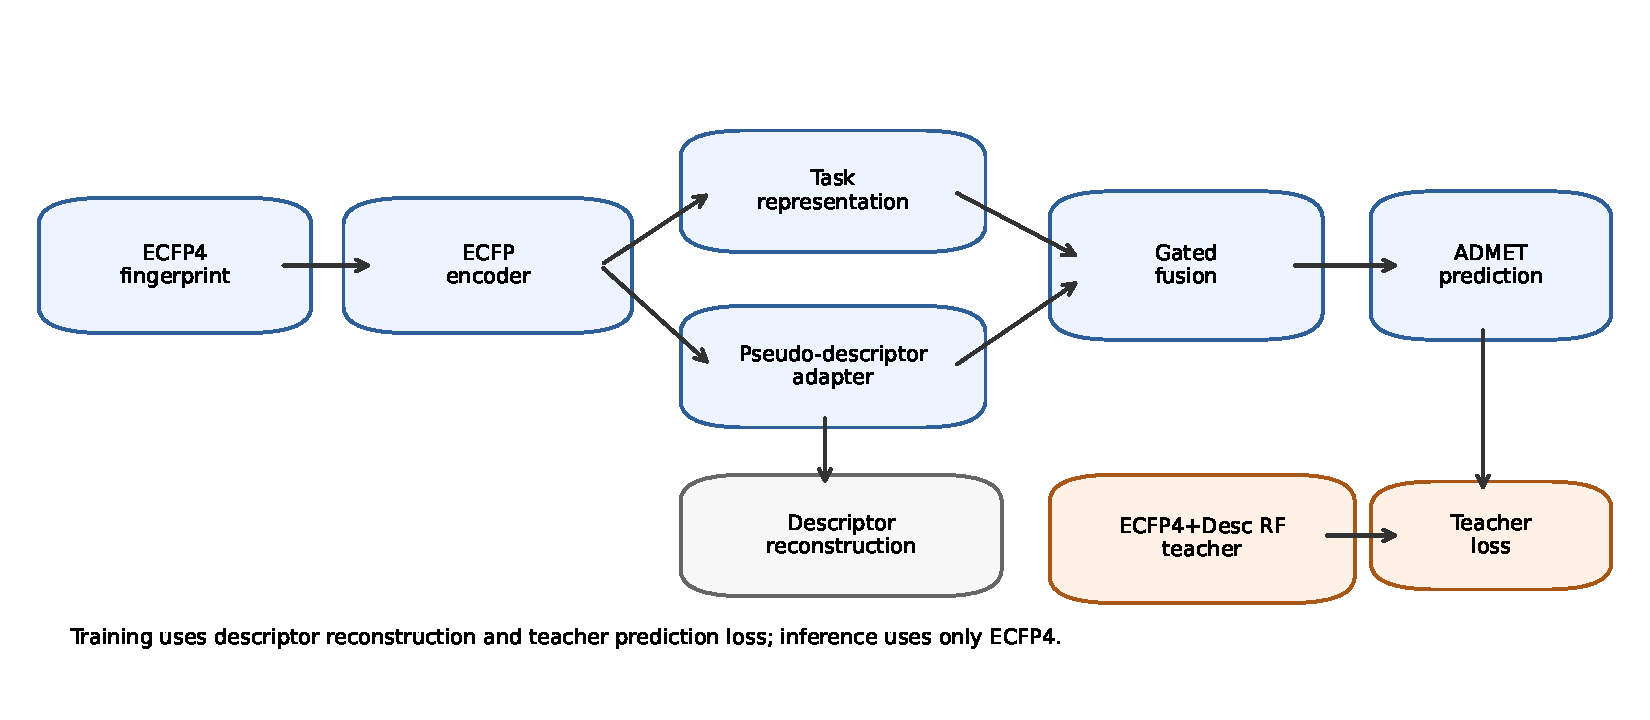
\includegraphics[width=\linewidth]{../paper_figures/fig1_method_diagram.pdf}
  \caption{Descriptor-Teacher AdapterFusion. Training uses descriptor
  reconstruction and teacher prediction distillation from an ECFP4+descriptor
  random forest. Inference uses only ECFP4.}
  \label{fig:method}
\end{figure}

\section{Experiments}

\subsection{Datasets and protocol}

The main regression benchmark includes five TDC ADMET tasks: Caco-2
permeability, lipophilicity, aqueous solubility, volume of distribution, and
plasma protein binding. Supplementary classification experiments cover five
standard binary ADMET endpoints. The main claims are restricted to regression
tasks because the distillation signal is more consistent there.

Each dataset is evaluated with training ratios of 10\%, 20\%, and 50\%. Each
setting is run with seeds 42, 123, and 3407. All models use the same
dataset-ratio-seed splits. Descriptor scalers are fit only on the training
split and then applied to validation and test splits.

\subsection{Baselines and metrics}

We compare ECFP4 MLP, ECFP4 MLP with descriptor prediction, AdapterFusion,
descriptor-concatenation MLP, ECFP4 random forest, descriptor random forest,
ECFP4+descriptor random forest, and Descriptor-Teacher AdapterFusion.
Descriptor-concatenation and descriptor random forest models use descriptors at
inference and should be interpreted as descriptor-access controls rather than
ECFP-only students.

Regression tasks use MAE and RMSE, with RMSE as the primary metric.
Classification tasks use ROC-AUC and PR-AUC and are reported only as
supplementary reference results. All tables report mean$\pm$standard deviation
over three seeds.

\section{Results}

\subsection{Main regression results}

\begin{table*}[t]
\centering
\small
\caption{Main low-resource regression ADMET results. Values are test RMSE mean$\pm$std over three seeds; lower is better. $\Delta$ is distilled AdapterFusion minus base AdapterFusion, so negative values indicate improvement.}
\label{tab:main_regression}
\resizebox{\textwidth}{!}{%
\begin{tabular}{llccccc}
\toprule
Dataset & Train \% & DescPred & AdapterFusion & ECFP4+Desc RF & Distilled AdapterFusion & $\Delta$ \\
\midrule
caco2\_wang & 10 & 3.3584$\pm$0.1667 & 1.7702$\pm$0.0304 & 0.5535$\pm$0.0017 & 1.7725$\pm$0.0497 & 0.0023 \\
caco2\_wang & 20 & 1.6383$\pm$0.0859 & 0.9541$\pm$0.0563 & 0.4691$\pm$0.0083 & 0.9459$\pm$0.0362 & -0.0081 \\
caco2\_wang & 50 & 0.7613$\pm$0.0784 & 0.6775$\pm$0.0995 & 0.4252$\pm$0.0121 & 0.6265$\pm$0.0508 & -0.0510 \\
lipophilicity\_astrazeneca & 10 & 1.2638$\pm$0.0440 & 1.2325$\pm$0.0114 & 1.0635$\pm$0.0011 & 1.2058$\pm$0.0219 & -0.0267 \\
lipophilicity\_astrazeneca & 20 & 1.1232$\pm$0.0275 & 1.0960$\pm$0.0132 & 0.9858$\pm$0.0015 & 1.0903$\pm$0.0083 & -0.0057 \\
lipophilicity\_astrazeneca & 50 & 1.0013$\pm$0.0082 & 0.9736$\pm$0.0059 & 0.9184$\pm$0.0012 & 0.9605$\pm$0.0057 & -0.0130 \\
solubility\_aqsoldb & 10 & 1.8330$\pm$0.0212 & 1.7832$\pm$0.0151 & 1.4996$\pm$0.0059 & 1.7906$\pm$0.0205 & 0.0074 \\
solubility\_aqsoldb & 20 & 1.7247$\pm$0.0477 & 1.7117$\pm$0.0125 & 1.3951$\pm$0.0021 & 1.7027$\pm$0.0288 & -0.0090 \\
solubility\_aqsoldb & 50 & 1.6411$\pm$0.0166 & 1.6107$\pm$0.0088 & 1.3397$\pm$0.0057 & 1.5963$\pm$0.0087 & -0.0144 \\
vdss\_lombardo & 10 & 5.4896$\pm$0.0889 & 5.4563$\pm$0.0463 & 5.2699$\pm$0.0051 & 5.4187$\pm$0.0199 & -0.0376 \\
vdss\_lombardo & 20 & 5.5751$\pm$0.1937 & 5.5086$\pm$0.1260 & 5.2805$\pm$0.0220 & 5.6795$\pm$0.0473 & 0.1709 \\
vdss\_lombardo & 50 & 5.3722$\pm$0.0619 & 5.2838$\pm$0.0352 & 5.0729$\pm$0.0257 & 5.3103$\pm$0.0309 & 0.0265 \\
ppbr\_az & 10 & 65.1399$\pm$20.3123 & 18.1281$\pm$0.1596 & 14.2419$\pm$0.0867 & 17.5888$\pm$0.2565 & -0.5393 \\
ppbr\_az & 20 & 26.9134$\pm$2.7840 & 16.6702$\pm$0.3270 & 13.7317$\pm$0.0288 & 16.4194$\pm$1.1199 & -0.2508 \\
ppbr\_az & 50 & 15.3150$\pm$0.3506 & 14.9058$\pm$0.5019 & 13.3106$\pm$0.0968 & 14.6711$\pm$0.7282 & -0.2347 \\
\bottomrule
\end{tabular}%
}
\end{table*}


Table~\ref{tab:main_regression} shows the main low-resource regression results.
Descriptor-access random forests remain strong, confirming that descriptor
information is predictive for ADMET properties. Among ECFP-only neural models,
AdapterFusion is consistently stronger than simple descriptor prediction on
the regression tasks, supporting the hypothesis that descriptor knowledge is
better transferred through a structured pseudo-descriptor adapter than through
a plain auxiliary descriptor head.

Teacher distillation further improves AdapterFusion. With
$\lambda_{\mathrm{distill}}=1.0$, distilled AdapterFusion improves over base
AdapterFusion in 11/15 regression settings, with a mean RMSE delta of -0.0656.
The gains are most visible in settings where the descriptor-access teacher has
a large advantage over the ECFP-only student, such as \texttt{ppbr\_az}. The
distilled student remains below the descriptor-access RF teacher in most
settings, so the result should be interpreted as partial descriptor knowledge
transfer, not replacement of descriptor-access baselines.

\begin{figure}[t]
  \centering
  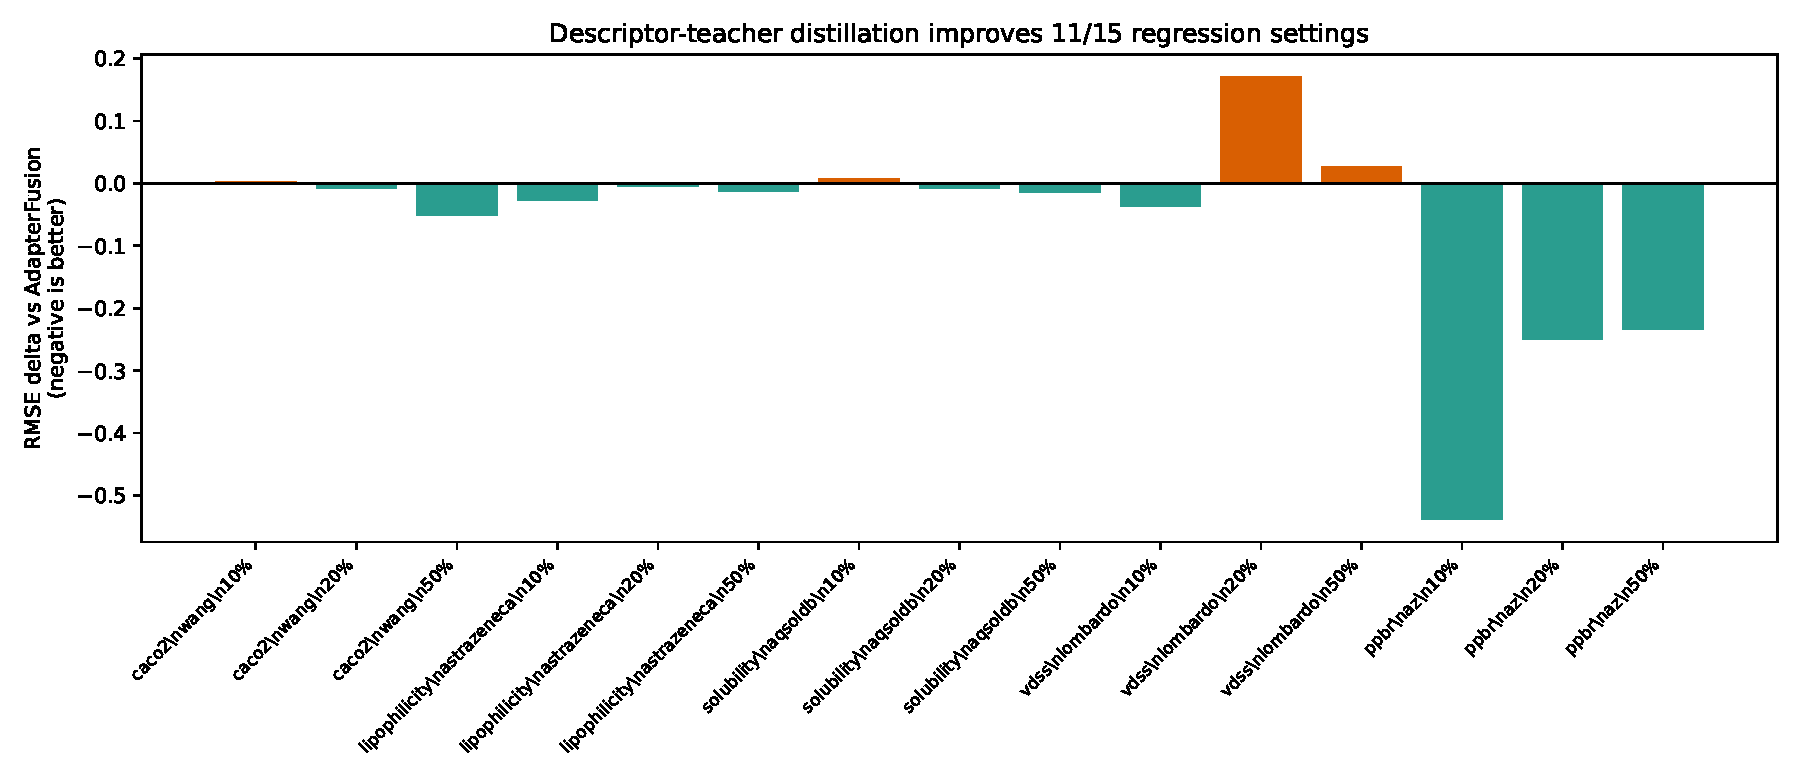
\includegraphics[width=\linewidth]{../paper_figures/fig2_distillation_delta.pdf}
  \caption{RMSE delta of distilled AdapterFusion relative to base
  AdapterFusion. Negative values indicate improvement. Fixed
  $\lambda_{\mathrm{distill}}=1.0$ improves 11/15 regression settings.}
  \label{fig:delta}
\end{figure}

\subsection{Lambda sensitivity}

\begin{table}[t]
\centering
\small
\caption{Fixed distillation lambda ablation over 15 regression dataset-ratio settings. Negative mean delta indicates improvement over base AdapterFusion.}
\label{tab:lambda_summary}
\begin{tabular}{lccc}
\toprule
$\lambda_{distill}$ & Complete & Beats Adapter & Mean $\Delta$ \\
\midrule
0.01 & 15/15 & 8/15 & 0.0075 \\
0.1 & 15/15 & 8/15 & -0.0221 \\
0.3 & 15/15 & 10/15 & -0.0046 \\
1.0 & 15/15 & 11/15 & -0.0656 \\
\bottomrule
\end{tabular}
\end{table}


Table~\ref{tab:lambda_summary} summarizes the fixed distillation lambda sweep.
The strongest global fixed value is $\lambda_{\mathrm{distill}}=1.0$. Smaller
lambdas can be better for individual settings, but they do not improve
aggregate performance. Validation-selected lambda is useful as an analysis but
beats fixed $\lambda_{\mathrm{distill}}=1.0$ in only 2/15 settings, while still
beating base AdapterFusion in 12/15 settings.

\begin{figure}[t]
  \centering
  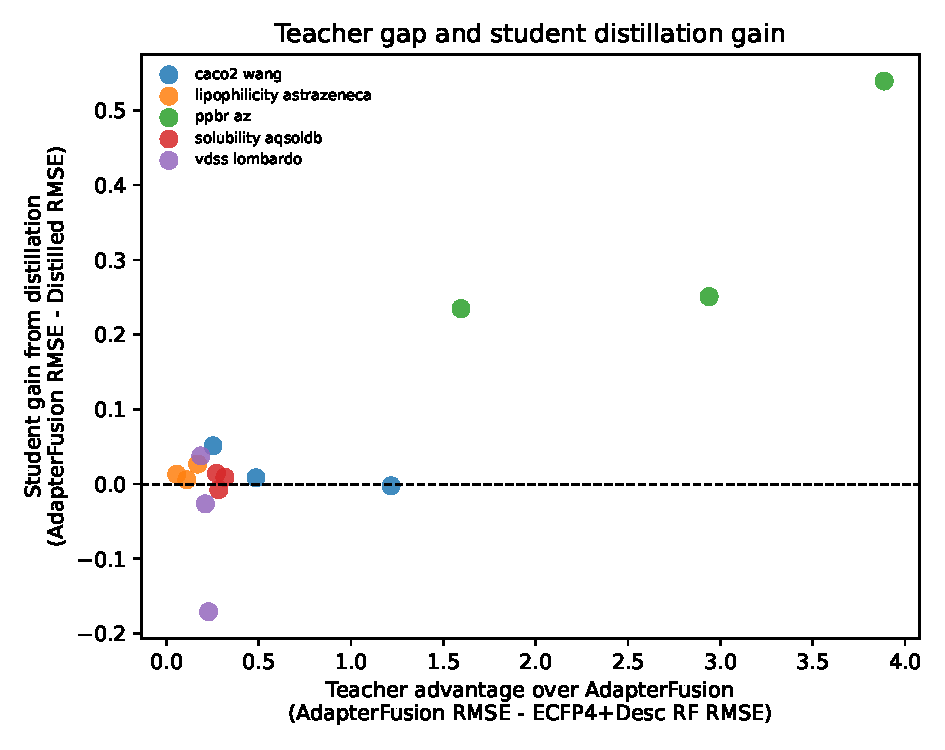
\includegraphics[width=0.82\linewidth]{../paper_figures/fig3_teacher_gap_gain.pdf}
  \caption{Relationship between descriptor-teacher advantage and student gain
  from distillation. Positive student gain means the distilled student has
  lower RMSE than base AdapterFusion.}
  \label{fig:teacher_gap}
\end{figure}

\subsection{Adaptive weighting as a negative ablation}

\begin{table}[t]
\centering
\small
\caption{Adaptive teacher-weighting negative ablation. The validation-advantage rule improves over base AdapterFusion in some settings, but is weaker than fixed strong distillation.}
\label{tab:adaptive_summary}
\begin{tabular}{lc}
\toprule
Comparison & Result \\
\midrule
Adaptive beats base AdapterFusion & 9/15 \\
Adaptive beats fixed $\lambda=1.0$ & 3/15 \\
Adaptive beats best fixed lambda & 1/15 \\
Mean $\Delta$ vs fixed $\lambda=1.0$ & 0.0817 \\
\bottomrule
\end{tabular}
\end{table}


Table~\ref{tab:adaptive_summary} summarizes the validation teacher-advantage
adaptive weighting rule. The adaptive rule improves over base AdapterFusion in
9/15 settings, but beats fixed $\lambda_{\mathrm{distill}}=1.0$ in only 3/15
settings and beats the best fixed lambda in only 1/15 settings. Its mean RMSE
delta relative to fixed $\lambda_{\mathrm{distill}}=1.0$ is 0.0817, indicating
worse average performance. This negative result shows that raw validation
teacher advantage is not a sufficient reliability signal for adaptive
distillation.

\subsection{Classification reference}

Classification results are reported as supplementary results. They are less
stable than the regression results, and descriptor-access controls are often
strong. We therefore do not use classification results as the main evidence for
Descriptor-Teacher AdapterFusion.

\section{Discussion}

The experiments support a controlled descriptor-guided transfer story.
Descriptor information is valuable, and descriptor-access baselines remain
strong. The contribution is not to replace descriptor-access random forests,
but to show that descriptor-access knowledge can partially improve an ECFP-only
neural student under low-resource regression ADMET settings.

AdapterFusion improves over plain descriptor prediction, suggesting that the
structure of auxiliary transfer matters. Teacher distillation then provides an
additional improvement by aligning the ECFP-only student with predictions from
a descriptor-access random forest teacher. The lambda sweep shows that stronger
teacher supervision is generally useful, with $\lambda_{\mathrm{distill}}=1.0$
as the best fixed global setting. However, the dataset-specific best lambda
varies, and neither validation-selected lambda nor the tested adaptive rule
clearly improves over the fixed setting.

\section{Limitations}

This work has several limitations. First, the main claim is restricted to
regression ADMET tasks. Classification results are included only as
supplementary evidence because improvements are less consistent. Second, the
student model is lightweight and ECFP-based; the method has not yet been tested
with large pretrained molecular encoders. Third, descriptor-access random
forests remain stronger than the distilled student in most settings. Finally,
the adaptive teacher-weighting strategy tested here is simple and negative;
more principled sample-level or learned teacher weighting may be needed.

\section{Conclusion}

We presented Descriptor-Teacher AdapterFusion, a lightweight
descriptor-guided multi-to-uni transfer method for low-resource regression
ADMET prediction. The method trains an ECFP-only AdapterFusion student with
descriptor reconstruction and teacher prediction distillation from an
ECFP4+descriptor random forest. The main fixed setting,
$\lambda_{\mathrm{distill}}=1.0$, improves AdapterFusion in 11/15 regression
dataset-ratio settings. At the same time, descriptor-access random forest
baselines remain stronger, so the appropriate conclusion is controlled
descriptor knowledge transfer rather than overall ADMET state-of-the-art
performance.

\bibliographystyle{plainnat}
\bibliography{references}

\end{document}
